%#! platex main.tex

%======================================================================
\chapter{提案手法}

本章では, ワイヤレスイヤホンに搭載されたマイクを使用して, 録音した食事中の音から食品認識と咀嚼検出を行う手法について詳述する. 咀嚼音には食材の硬さや質感, 噛むタイミングなどの情報が含まれていると考える. 例えば, ポテトチップスの咀嚼音は特有であり, その音を聞くだけでポテトチップスであると認識し, 咀嚼のタイミングを推測することが可能である.

食事中の音には, 咀嚼音の他に, 皿や箸などのカトラリによる音や環境ノイズも含まれている. 食品認識や咀嚼検出を高い精度で行うためには, これらのノイズを減らし, 咀嚼音のみを効果的に抽出することが重要なステップとなる. この点で, ワイヤレスイヤホンは耳に装着され, 咀嚼音が発生する口に近い位置にあるため, 咀嚼音の要素を多く含んだ音を記録することに優位性を持つ.

食品推定では, 食事中の音データを0.5秒のセグメントに分割し, これらのセグメントをメルスペクトログラムに変換し, 畳み込みニューラルネットワーク(CNN)での学習を通じて食品推定モデルを生成する. 咀嚼検出についても同様のアプローチをとり, セグメントをメルスペクトログラムに変換し, CNNで学習を行い, 咀嚼検出モデルを生成する. 咀嚼検出における正解ラベルは, セグメント内に咀嚼タイムスタンプが1つ以上存在する場合を「咀嚼あり」, 存在しない場合を「咀嚼なし」とする.

学習に使用するデータセットは, 前章で説明したデータ収集アプリケーションによって収集されたデータを使用する. このデータセットには, 食事中の音データと正解データが含まれる. ただし, 食事中の音データは1ファイル1品のみであり, 正解データには食品の種類と咀嚼タイムスタンプが含まれる. 図\ref{fig:wave-sample}にポテトチップスのデータの例を示す. これらのデータを用いて, 精度の高い食品認識と咀嚼検出モデルの構築を目指す.

\begin{figure}[t]
    \begin{center}
        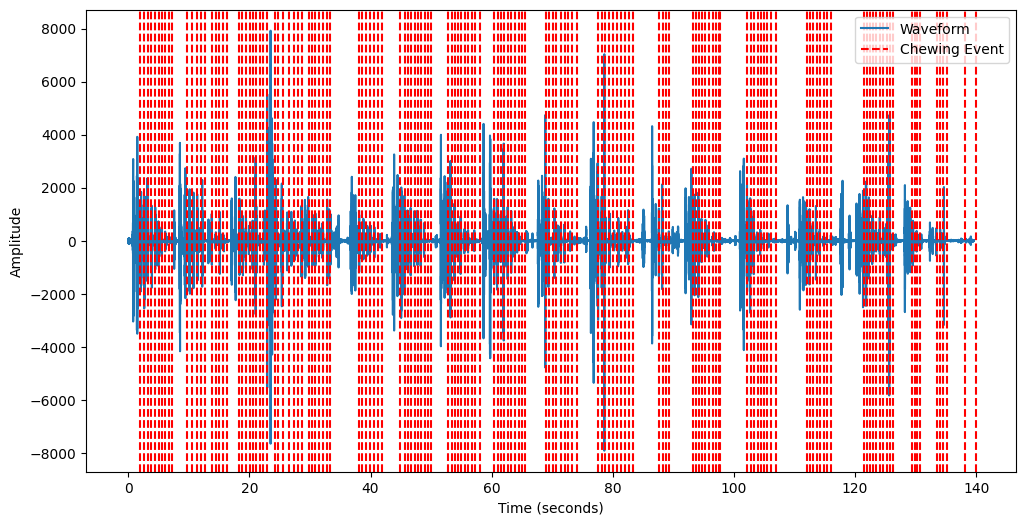
\includegraphics[clip,  width=0.95\hsize]{img/wave-sample.png}
        \caption{データ収集アプリケーションによって収集されたデータの例}
        \label{fig:wave-sample}
    \end{center}
\end{figure}

%----------------------------------------------------------------------
\section{食品推定}

食事中の録音データをメルスペクトログラムに変換し, 畳み込みニューラルネットワークによる学習を行うことで, 食事内容推定モデルを生成する. メルスペクトログラムを用いてCNNで音声分類を行うと従来の手法よりも精度が出ることが言われているため\cite{Dossou_2021_ICCV}, 本研究でもこの手法を採用する.
食事中に発生する音をウィンドウ幅$500ms$, オーバーラップ率$0.75$のスライディングウィンドウで部分時系列データに分割する. ただし, 最大信号強度が$-65dBFS$以下のデータと音の長さが$500ms$に満たないものは除外する. 特徴抽出のために, スライディングウィンドウでセグメントされた音データに対して, メルスペクトログラムを算出する. これらのデータを訓練データ$90\%$とテストデータ$10\%$に分割し, 訓練データを用いて畳み込みニューラルネットワークCNNを学習させる. CNNには4つの畳み込み層を使用し, 畳み込み層の後に一つの最大値プーリング層とドロップアウト層を使用する. 最後の層はソフトマックス層である. 最終的に, テストデータを用いて学習済みモデルの精度評価を行う.

%----------------------------------------------------------------------
\section{咀嚼検出}

音声信号処理においてオンセット検出は一般的な手法であり, スペクトルエネルギ分布からピークを検出することで, 音楽イベントを自動で検出することができる. 本稿でも, 咀嚼イベントの検出にオンセット検出を採用する. 食事中の音をメルスペクトログラムに変換し, 各時間軸毎の全ての周波数帯の信号強度の平均を取り, ピークを検出することで, 咀嚼の検出を行う. 図\ref{fig:peak-sample}にピーク検出の例を示す. 評価については, 10秒間の音データに対して被験者がカウントした咀嚼回数とピーク検出回数との間の平均絶対値誤差$MAE$を算出する. $MAE$の算出式は以下に示す.

\begin{equation}
    \text{MAE} = \frac{1}{n} \sum_{i=1}^{n} | y_i - \hat{y}_i |
\end{equation}

% 以下はRefTeX用
%%% Local Variables:
%%% mode: yatex
%%% TeX-master: "main"
%%% End:
